%% Part of Stellarium User Guide
%% Status: 2015-12-30 Some parts collected from wiki.
%%         2016-04-05 GZ changed to have 1 chapter per plugin for a better structure. This file may be split up later. 
%% TODO: All plugins! And give a better structure than just by alphabet.
%%         2016-04-16 split plugin part to topical chapters.

\chapter{Interface Extensions}
\label{ch:plugins:Interfaces}

Most users will soon be familiar with the usual user interface. A few
plugins are available which extend the regular user interface with a
few small additions which are presented first.  However, some
applications and installations of Stellarium require completely
different user interfaces. Mostly, these serve to avoid showing the
user interface panels to an audience, be that in your astronomy club
presentations, a domed planetarium or in a museum installation.


\section{Angle Measure Plugin}
\label{sec:plugins:AngleMeasure}

\begin{quotation}\small
\noindent\emph{goes misty eyed}\\ 
I recall measuring the size of the Cassini Division when I was a student.
It was not the high academic glamor one might expect\ldots It was cloudy\ldots
It was rainy\ldots The observatory lab had some old scopes set up at one
end, pointing at a \emph{photograph} of Saturn at the other end of the
lab. We measured. We calculated. We wished we were in Hawaii. A picture
is worth a thousand words.
\end{quotation}

%\url{http://porpoisehead.net/images/plugin-angle-measure.jpg}

\noindent The Angle Measure plugin is a small tool which is used to measure the
angular distance between two points on the sky. 


%\subsection{Using the plugin}
%\label{sec:plugins:AngleMeasure:using}

\begin{enumerate}
\item Enable the tool by clicking the tool-bar button, or by pressing
  \key{\ctrl+A}. A message will appear at the bottom of the screen to
  tell you that the tool is active.
\item Drag a line from the first point to the second point using the
  left mouse button
\item To clear the measurement, click the right mouse button
\item To deactivate the angle measure tool, press the tool-bar button
  again, or press \key{\ctrl+A} on the keyboard.
\end{enumerate}

\noindent In the configuration dialog, you can configure if you want to have
distances given on the rotating sphere, or in horizontal
(alt-azimuthal) coordinates. You can also link one point to the
resting horizon, the other to the sky and observe how angles change.

\newpage

\section{Compass Marks Plugin}
\label{sec:plugins:CompassMarks}

%\url{http://porpoisehead.net/images/plugin-compass-marks.jpg}

Stellarium helps the user get their bearings using the cardinal point
feature -- the North, South, East and West markers on the horizon.
Compass Marks takes this idea and extends it to add markings every few
degrees along the horizon, and includes compass bearing values in
degrees.

When activated (see section~\ref{sec:Plugins:EnablingPlugins}), there
is a tool bar button \guibutton{0.6}{bt_compass_off} for toggling the
compass markings.  Note that when you enable compass marks, the
cardinal points will be turned off.

%% TODO/FIXME?: The following is not true for current pre-0.15:
%You can have both active at once, but there is a small
%bug which means you have to press \key{Q} \emph{two times} to
%re-enable cardinal points after enabling the compass markings.


\newpage
\section{Equation of Time Plugin}
\label{sec:plugins:EquationOfTime}

%% The figure just reproduces most of the text. I (GZ) regard it not so necessary. 
%\begin{figure}[h]
%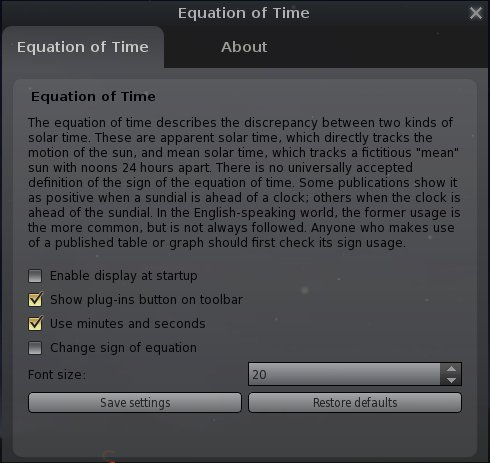
\includegraphics[width=\textwidth]{EquationOfTime-plugin.jpg}
%\label{fig:EqOfTime}
%\caption{Interface of Equation of Time plugin}
%\end{figure}

\noindent The Equation of Time plugin shows the solution of the equation of time. % (Fig.~\ref{fig:EqOfTime}).
This describes the discrepancy between two kinds of
solar time:
\begin{description}
\item[Apparent solar time] directly tracks the motion of the sun. Most sundials show this time.
\item[Mean solar time] tracks a fictitious ``mean'' sun with noons 24 hours apart. 
\end{description}

There is no universally accepted definition of the sign of the
equation of time. Some publications show it as positive when a sundial
is ahead of a clock; others when the clock is ahead of the sundial. In
the English-speaking world, the former usage is the more common, but
is not always followed. Anyone who makes use of a published table or
graph should first check its sign usage.

If enabled (see section~\ref{sec:Plugins:EnablingPlugins}), click on
the Equation of Time button \guibutton{0.6}{bt_EquationOfTime_72dpi}
on the bottom toolbar to display the value for the equation of time on
top of the screen.


\subsection{Section \big[EquationOfTime\big] in config.ini file}
\label{sec:plugins:EquationOfTime:config}

You can edit \file{config.ini} file by yourself for changes of the
settings for the Equation of Time plugin -- just make it carefully!

\begin{longtabu} to \textwidth {l|l|X}\toprule
\emph{ID}            & \emph{Type} & \emph{Description}\\\midrule
enable\_at\_startup  & bool & Display solution of the equation of time at startup of the planetarium\\\midrule
flag\_use\_ms\_format & bool & Set format for the displayed solution - minutes and seconds and decimal minutes\\\midrule
flag\_use\_inverted\_value & bool & Change sign of the equation of time \\\midrule
flag\_show\_button & bool & Enable displaying plugin button on the bottom toolbar\\\midrule
text\_color & R,G,B & Color of font for the displayed solution of the equation of time\\\midrule
font\_size & int & Font size for the displayed solution of the equation of time \\\bottomrule
\end{longtabu}



\newpage

\section{Field of View Plugin}
\label{sec:plugins:FieldOfView}

\begin{figure}[ht]
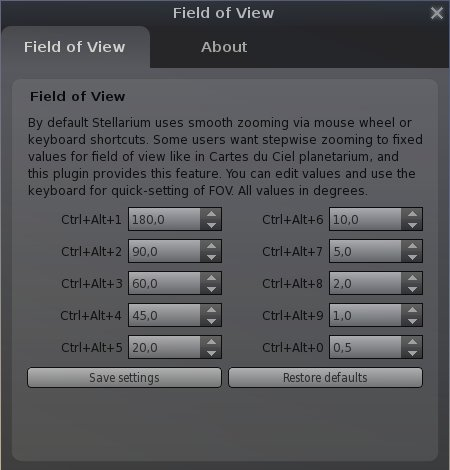
\includegraphics[width=\textwidth]{FOV-plugin.jpg}
\label{fig:plugins:FieldOfView}
\caption{Configuration dialog of Field of View plugin}
\end{figure}

\noindent By default Stellarium uses smooth zooming via mouse wheel or
keyboard shortcuts. Some users may want stepwise zooming to fixed
values for field of view like in the \program{Cartes du
  Ciel}\footnote{SkyChart / Cartes du Ciel planetarium:
  \url{http://www.ap-i.net/skychart/en/start}} planetarium program,
and this plugin provides this feature. You can edit values and use the
keyboard for quick-setting of FOV. All values in degrees.

%\section{Using the Field of View plugin}
%\label{sec:plugins:FieldOfView:using}

\begin{enumerate}
\item Enable the tool by configuring it to ``Load at startup''.
\item Press shortkeys for quick changes of FOV.
\end{enumerate}

\subsection{Section \big[FOV\big] in config.ini file}
\label{sec:plugins:FieldOfView:config}

You can configure the plugin with its dialog (Fig.~\ref{fig:plugins:FieldOfView}) or edit
\file{config.ini} file by yourself for changes of the settings for the
Field of View plugin -- just make it carefully!

\begin{longtabu} to \textwidth {l|l|r|X}\toprule
\emph{ID} & \emph{Type} & \emph{Default} & \emph{Description}\\\midrule
fov\_quick\_0  & float & 0.5& Value of FOV for the shortcut \key{\ctrl+\Alt+0} \\\midrule
fov\_quick\_1  & float &180 & Value of FOV for the shortcut \key{\ctrl+\Alt+1} \\\midrule
fov\_quick\_2  & float & 90 & Value of FOV for the shortcut \key{\ctrl+\Alt+2} \\\midrule
fov\_quick\_3  & float & 60 & Value of FOV for the shortcut \key{\ctrl+\Alt+3} \\\midrule
fov\_quick\_4  & float & 45 & Value of FOV for the shortcut \key{\ctrl+\Alt+4} \\\midrule
fov\_quick\_5  & float & 20 & Value of FOV for the shortcut \key{\ctrl+\Alt+5} \\\midrule
fov\_quick\_6  & float & 10 & Value of FOV for the shortcut \key{\ctrl+\Alt+6} \\\midrule
fov\_quick\_7  & float &  5 & Value of FOV for the shortcut \key{\ctrl+\Alt+7} \\\midrule
fov\_quick\_8  & float &  2 & Value of FOV for the shortcut \key{\ctrl+\Alt+8} \\\midrule
fov\_quick\_9  & float &  1 & Value of FOV for the shortcut \key{\ctrl+\Alt+9} \\\bottomrule
\end{longtabu}

\newpage

\section{Pointer Coordinates Plugin}
\label{sec:plugins:PointerCoordinates}


\begin{figure}[th]
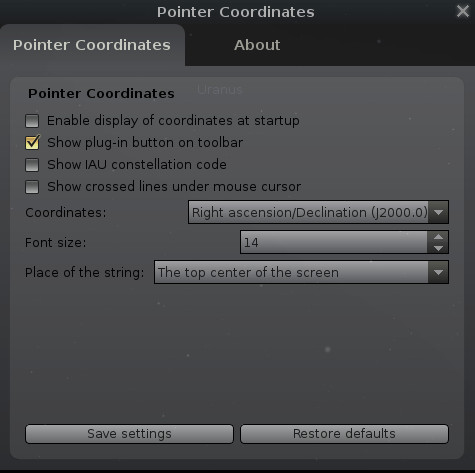
\includegraphics[width=\textwidth]{PointerCoordinates-plugin.jpg}
\label{fig:PointerCoordinates}
\caption{Interface of Pointer Coordinates plugin}
\end{figure}

\noindent The Pointer Coordinates plugin shows the coordinates of the mouse pointer.
If enabled, click on the plugin button \guibutton{0.6}{bt_PointerCoordinates_Off} on the bottom toolbar to display the coordinates of the mouse pointer.

\subsection{Section \big[PointerCoordinates\big] in config.ini file}
\label{sec:plugins:PointerCoordinates:config}

You can edit \file{config.ini} file by yourself for changes of the
settings for the Pointer Coordinates plugin -- just make it carefully!

\begin{longtabu} to \textwidth {l|l|X}\toprule
\emph{ID}            & \emph{Type} & \emph{Description}\\\midrule
enable\_at\_startup  & bool & Enable displaying coordinates of the mouse pointer at startup of the plugin\\\midrule
flag\_show\_button   & bool & Enable showing the button of the plugin on bottom toolbar\\\midrule
text\_color          & R,G,B & Color for text with coordinates of the mouse pointer \\\midrule
font\_size           & int & Font size for the displayed coordinates of the mouse pointer \\\midrule
current\_displaying\_place  & string & Specifies the place of displaying coordinates of the mouse pointer. \textit{Possible values}: \keymap{TopRight}, \keymap{TopCenter}, \keymap{RightBottomCorner}, \keymap{Custom}. \textit{Default value}: \keymap{TopRight}. \\\midrule
current\_coordinate\_system & string & Specifies the coordinate system. \textit{Possible values}: \keymap{RaDecJ2000}, \keymap{RaDec}, \keymap{HourAngle}, \keymap{Ecliptic}, \keymap{AltAzi}, \keymap{Galactic}. \textit{Default value}: \keymap{RaDecJ2000}. \\\midrule
custom\_coordinates  & int,int & Specifies the screen coordinates of the custom place for displaying coordinates of the mouse pointer \\\bottomrule
\end{longtabu}




\newpage

\section{Text User Interface}
\label{sec:plugins:TextUserInterface}

%\url{http://porpoisehead.net/images/plugin-tui.jpg}

Older versions of Stellarium used to have a little menu system which
was controlled by the cursor keys. This was used primarily by
planetarium system operators to change settings, run scripts and so
on. In the 0.10.x series, this function vanished as we totally
re-designed the user interface. This plugin re-implements the ``TUI'',
as it was known. A full list of the commands for the TUI plugin is
given in section~\ref{sec:plugins:TUI:commands}. Given that color
configuration for lines and texts cannot be found elsewhere, an interesting part is the
way to interactively select colors in this menu.


\subsection{Using the Text User Interface}
\label{sec:plugins:TUI:using}

\begin{enumerate}
\item Activate the text menu using the \key{\Alt+T} key.\footnote{This
    used to be hard-coded to \key{M} before version 0.15, but
    \key{\Alt+T} runs parallel with \key{\ctrl+T} for switching the GUI
    panels, and frees up \key{M} for the Milky Way. The \key{\Alt+T}
    keybinding is hardcoded, i.e., cannot be reconfigured by the
    user.}
\item
  Navigate the menu using the cursors keys.
\item
  To edit a value, press the right cursor until the value you wish to
  change it highlighted with \textgreater{} and \textless{} marks, e.g.\
  \textgreater{}3.142\textless{}. Then press the up and down cursors to
  change the value. You may also type in a new value with the other keys
  on the keyboard.
\end{enumerate}

%% TODO: Walk through and make sure this rundown is correct:

\subsection{TUI Commands}
\label{sec:plugins:TUI:commands}
\begin{longtabu} to \textwidth {l|l|X}
\toprule
1   & Set Location & (menu group)\\\midrule
1.1 & Latitude & Set the latitude of the observer in degrees\\\midrule
1.2 & Longitude & Set the longitude of the observer in degrees\\\midrule
1.3 & Altitude (m) & Set the altitude of the observer in meters\\\midrule
1.4 & Solar System Body & Select the solar system body on which the observer is\\\midrule
2   & Set Time & (menu group)\\\midrule
2.1 & Sky Time & Set the time and date for which Stellarium will generate the view\\\midrule
2.2 & Set Time Zone & Set the time zone. Zones are split into continent or region, and then by city or province\\\midrule
2.3 & Days keys & The setting ``Calendar'' makes the - = {[} {]} and keys change the date value by calendar days (multiples of 24 hours). 
                  The setting ``Sidereal day'' changes these keys to change the date by sidereal days\\\midrule
2.4 & Preset Sky Time & Select the time which Stellarium starts with (if the ``Sky Time At Start-up'' setting is ``Preset Time''\\\midrule
2.5 & Sky Time At Start-up & The setting ``Actual Time'' sets Stellarium's time to the computer clock when Stellarium runs. 
                             The setting ``Preset Time'' selects a time set in menu item ``Preset Sky Time''\\\midrule
2.6 & Time Display Format & Change how Stellarium formats time values. ``system default'' takes the format from the computer settings, 
                            or it is possible to select 24 hour or 12 hour clock modes\\\midrule
2.7 & Date Display Format & Change how Stellarium formats date values. ``system default'' takes the format from the computer settings, 
                            or it is possible to select ``yyyymmdd'', ``ddmmyyyy'' or ``mmddyyyy'' modes\\\midrule
3    & General & (menu group)\\\midrule
3.1  & Sky Culture  & Select the sky culture to use (changes constellation lines, names, artwork)\\\midrule
3.2  & Sky Language & Change the language used to describe objects in the sky\\\midrule
4    & Stars & (menu group)\\\midrule
4.1  & Show & Turn on/off star rendering\\\midrule
4.2  & Star Magnitude Multiplier & Can be used to change the brightness of the stars which are visible at a given zoom level. 
                                   This may be used to simulate local seeing conditions - the lower the value, the less stars will be visible\\\midrule
4.3  & Maximum Magnitude to Label & Changes how many stars get labelled according to their apparent magnitude (if star labels are turned on)\\\midrule
4.4  & Twinkling & Sets how strong the star twinkling effect is - zero is off, the higher the value the more the stars will twinkle.\\\midrule
5    & Colors & (menu group)\\\midrule
5.1  & Constellation Lines         & Changes the colour of the constellation lines\\\midrule
5.2  & Constellation Names         & Changes the colour of the labels used to name stars\\\midrule
5.3  & Constellation Art Intensity & Changes the brightness of the constellation artconstellation art\\\midrule
5.4  & Constellation Boundaries    & Changes the colour of the constellation boundary lines\\\midrule
5.5  & Cardinal Points & Changes the colour of the cardinal points markers\\\midrule
5.6  & Planet Names    & Changes the colour of the labels for planets\\\midrule
5.7  & Planet Orbits   & Changes the colour of the orbital guide lines for planets\\\midrule
5.8  & Planet Trails   & Changes the colour of the planet trails lines\\\midrule
5.9  & Meridian Line   & Changes the colour of the meridian line\\\midrule
5.10 & Azimuthal Grid  & Changes the colour of the lines and labels for the azimuthal grid\\\midrule
5.11 & Equatorial Grid & Changes the colour of the lines and labels for the equatorial grid\\\midrule
5.12 & Equator Line    & Changes the colour of the equator line\\\midrule
5.13 & Ecliptic Line   & Changes the colour of the ecliptic line\\\midrule
5.14 & Nebula Names    & Changes the colour of the labels for nebulae\\\midrule
5.15 & Nebula Circles  & Changes the colour of the circles used to denote the positions of nebulae (only when enabled int he configuration file, note this feature is off by default)\\\midrule
6   & Effects & (menu group)\\\midrule
6.1 & Light Pollution Luminance & Changes the intensity of the light pollution simulation\\\midrule
6.2 & Landscape & Used to select the landscape which Stellarium draws when ground drawing is enabled\\\midrule
6.3 & Manual zoom & Changes the behaviour of the \key{/} and \key{\textbackslash{}} keys. 
                    When set to ``No'', these keys zoom all the way to a level defined by object type (auto zoom mode). 
                    When set to ``Yes'', these keys zoom in and out a smaller amount and multiple presses are required\\\midrule
6.4 & Object Sizing Rule & When set to ``Magnitude'', stars are drawn with a size based on their apparent magnitude. 
                           When set to ``Point'' all stars are drawn with the same size on the screen\\\midrule
6.5 & Magnitude Sizing Multiplier & Changes the size of the stars when ``Object Sizing Rule'' is set to ``Magnitude''\\\midrule
6.6 & Milky Way intensity & Changes the brightness of the Milky Way texture\\\midrule
6.7 & Maximum Nebula Magnitude to Label & Changes the magnitude limit for labelling of nebulae\\\midrule
6.8 & Zoom Duration & Sets the time for zoom operations to take (in seconds)\\\midrule
6.9 & Cursor Timeout & Sets the number of seconds of mouse inactivity before the cursor vanishes\\\midrule
6.10 & Setting Landscape Sets Location & If ``Yes'' then changing the landscape will move the observer location to the location for that landscape (if one is known). 
                                         Setting this to ``No'' means the observer location is not modified when the landscape is changed.\\\midrule
7 & Scripts & (menu group)\\\midrule
7.1 & Local Script & Run a script from the scripts sub-directory of the User Directory or Installation Directory (see section~\ref{sec:FilesAndDirectories} (Files and Directories))\\\midrule
7.2 & CD/DVD Script          & Run a script from a CD or DVD (only used in planetarium set-ups)\\\midrule
8   & Administration         & (menu group)\\\midrule
8.1 & Load Default Configuration & Reset all settings according to the main configuration file\\\midrule
8.2 & Save Current Configuration as Default & Save the current settings to the main configuration file\\\midrule
8.3 & Shutdown               & Quit Stellarium\\\midrule
8.4 & Update me via Internet & Only used in planetarium set-ups\\\midrule
8.5 & Set UI Locale          & Change the language used for the user interface\\\bottomrule
\end{longtabu}

\newpage
\section{Remote Control}
\label{sec:plugin:RemoteControl}

[This will come as user documentation from SoCiS2015 work]


% \newpage
% \section{D-Bus Interface}
% \label{sec:plugin:DBus}
% 
% [This may come as user documentation from SoCiS2016 (?) work]


\newpage

\section{Solar System Editor Plugin}
\label{sec:plugins:SolarSystemEditor}
TODO...

\section{Timezone Configuration Plugin}
\label{sec:plufins:Timezones}
TODO...



%%% Local Variables: 
%%% mode: latex
%%% TeX-master: "guide"
%%% End: 

